\documentclass[11pt,a4paper]{article}

%%%%%%%%%%%%%%%%%%%%%%%%%%%%%%%%%%
% Encoding and language
\usepackage[utf8]{inputenc}
\usepackage[T1]{fontenc}
\usepackage[english]{babel}
\selectlanguage{English}

%%%%%%%%%%%%%%%%%%%%%%%%%%%%%%%%%%
% General packages
\usepackage{verbatim}
\usepackage[all]{xy}
\usepackage{float}
\usepackage{amsmath}
\usepackage{array}
\usepackage{listings}
\usepackage{xcolor}
\usepackage{setspace}
\usepackage{booktabs}
\usepackage{graphicx}
\usepackage{url}
\usepackage{lmodern}
\interfootnotelinepenalty=10000

%%%%%%%%%%%%%%%%%%%%%%%%%%%%%%%%%%
% Page layout
\usepackage{geometry}
\geometry{margin=2.5cm}

%%%%%%%%%%%%%%%%%%%%%%%%%%%%%%%%%%
% Hyperlinks
\usepackage[
    colorlinks=true,
    urlcolor=blue!50!black,
    linkcolor=black,
    citecolor=black
]{hyperref}

%%%%%%%%%%%%%%%%%%%%%%%%%%%%%%%%%%
% Bibliography
\usepackage[round]{natbib}

%%%%%%%%%%%%%%%%%%%%%%%%%%%%%%%%%%
% Fancy headers (ALL pages incl. title page)
\usepackage{fancyhdr}
\pagestyle{fancy}

\fancyhf{} % clear header/footer

\fancyhead[L]{zpn710, fps618, kvb125, xnc401 - everyone contributed equally}
\fancyhead[R]{February 2026}
\fancyfoot[C]{\thepage}

\renewcommand{\headrulewidth}{0.4pt}
\renewcommand{\footrulewidth}{0pt}

% IMPORTANT: make 'plain' style match 'fancy'
\fancypagestyle{plain}{
    \fancyhf{}
    \fancyhead[L]{zpn710, fps618, kvb125, xnc401 - everyone contributed equally}
    \fancyhead[R]{February 2026}
    \fancyfoot[C]{\thepage}
    \renewcommand{\headrulewidth}{0.4pt}
}

%%%%%%%%%%%%%%%%%%%%%%%%%%%%%%%%%%
% Listings styles
\lstdefinestyle{CStyle}{
    language=C,
    basicstyle=\small\ttfamily,
    keywordstyle=\color{blue},
    commentstyle=\color{green!40!black},
    stringstyle=\color{orange},
    numbers=left,
    numberstyle=\tiny,
    stepnumber=1,
    numbersep=5pt,
    backgroundcolor=\color{gray!5},
    frame=single,
    rulecolor=\color{black!30},
    captionpos=b,
    breaklines=true,
    breakatwhitespace=true,
    tabsize=4,
    showspaces=false,
    showstringspaces=false,
}

\definecolor{bluekeywords}{rgb}{0.13,0.13,1}
\definecolor{greencomments}{rgb}{0,0.5,0}
\definecolor{turqusnumbers}{rgb}{0.17,0.57,0.69}
\definecolor{redstrings}{rgb}{0.5,0,0}

\lstdefinelanguage{FSharp}{
    morekeywords={let,new,match,with,rec,open,module,namespace,type,of,member,and,for,in,do,begin,end,fun,function,try,mutable,if,then,else},
    keywordstyle=\color{bluekeywords},
    sensitive=false,
    morecomment=[l][\color{greencomments}]{///},
    morecomment=[l][\color{greencomments}]{//},
    morecomment=[s][\color{greencomments}]{{(*}{*)}},
    morestring=[b]",
    stringstyle=\color{redstrings}
}

%%%%%%%%%%%%%%%%%%%%%%%%%%%%%%%%%%
% Matrix spacing fix
\makeatletter
\renewcommand*\env@matrix[1][*\c@MaxMatrixCols c]{%
  \hskip -\arraycolsep
  \let\@ifnextchar\new@ifnextchar
  \array{#1}}
\makeatother

%%%%%%%%%%%%%%%%%%%%%%%%%%%%%%%%%%
% Graphics paths
\graphicspath{{figures/}{anotherFigureDirectory/}}

%%%%%%%%%%%%%%%%%%%%%%%%%%%%%%%%%%
% Title (no author/date under title)
\title{\LARGE \textbf{Handin 4 Numerical Optimization}}
\date{}

\makeatletter
\def\@maketitle{%
  \newpage
  \vskip 0em % ← space above title (adjust if you want)
  \begin{center}%
    {\LARGE \bfseries \@title \par}%
    \vskip 0.2em % ← space below title (THIS controls the gap)
  \end{center}%
}
\makeatother

%%%%%%%%%%%%%%%%%%%%%%%%%%%%%%%%%%
\begin{document}

\maketitle

\section{Introduction}

This report investigates the theoretical and practical performance of quasi-Newton methods, with focus on BFGS. We prove Q-superlinear convergence for a quadratic model under standard assumptions and implement BFGS with a strict Wolfe line-search and evaluate its performance against Newton methods on several test problems.

\section{Theory: Q-Superlinear Convergence for Quadratic Functions}

We consider the quadratic function
\[
f(x) = \tfrac12 x^T Q x + g^T x,
\qquad Q \in \mathbb{R}^{n\times n}, \quad Q \succ 0
\]
Then
\[
\nabla f(x) = Qx + g
\]
We set $B_k \to Q$ and define the iteration
\[
p_k = -B_k^{-1}\nabla f(x_k),
\qquad
x_{k+1} = x_k + p_k
\]

\paragraph{Gradient relation:} Using the quadratic structure we get
\[
\nabla f(x_{k+1})
= Q(x_k + p_k) + g
= \nabla f(x_k) + Qp_k
\]
Substituting $p_k = -B_k^{-1}\nabla f(x_k)$ gives
\[
\nabla f(x_{k+1})
= \nabla f(x_k) - Q B_k^{-1} \nabla f(x_k)
= (I - Q B_k^{-1}) \nabla f(x_k)
\]
Now we define
\[
R_k := I - Q B_k^{-1}
\]
Then
\[
\nabla f(x_{k+1}) = R_k \nabla f(x_k)
\]

\paragraph{Convergence of $R_k$:} Since $B_k \to Q$ and $Q$ is positive definite and therefore invertible, matrix inversion is continuous on invertible matrices, so
\[
B_k^{-1} \to Q^{-1}
\]
Therefore
\[
Q B_k^{-1} \to QQ^{-1} = I \quad \text{thus} \quad R_k = I - Q B_k^{-1} \to 0
\]

\paragraph{Q-superlinear convergence:} From the gradient relation we apply the operator norm\footnote{We use the operator norm here so that the inequality $\|R_k v\| \le \|R_k\|\,\|v\|$ holds. This was taught in the course \emph{Advanced Vector Spaces}. In finite dimensions, all norms are equivalent, so the convergence result is the same for any other norm (for example, the Euclidean norm).}
\[
\|\nabla f(x_{k+1})\|
= \|R_k \nabla f(x_k)\|
\le \|R_k\| \, \|\nabla f(x_k)\|
\]
The operator norm satisfies
\[
\|R_k\| = \max_i |\lambda_i(R_k)|
\]
where $\lambda_i(R_k)$ are the eigenvalues of $R_k$. Since $R_k \to 0$, all eigenvalues $\lambda_i(R_k) \to 0$, and therefore
\[
\|R_k\| \to 0
\]
Consequently
\[
\frac{\|\nabla f(x_{k+1})\|}{\|\nabla f(x_k)\|}
\le \|R_k\|
\to 0
\]
By definition, this proves that $\|\nabla f(x_k)\|$ converges to zero
\emph{Q-superlinearly}.


\section{Programming: Performance Analysis of BFGS}

\subsection{Verification of the Strict Wolfe Line Search}

To verify the correctness of our implementation of Algorithm~8, we designed systematic tests to ensure that all logical branches of the Wolfe line-search were triggered and behaved correctly. The purpose of the line search is to compute a step length $\alpha_k$ 
satisfying the strong Wolfe conditions. In particular, the curvature condition guarantees $s_k^T y_k > 0$, which ensures that the BFGS update remains well-defined and preserves positive definiteness:
\[
p_k^T \nabla f(x_k + \alpha_k p_k)
\ge c_2\, p_k^T \nabla f(x_k)
\]
We performed the main verification on $f_3$, which exhibits nontrivial curvature behaviour. By varying the initial step length and using different starting points, we forced the algorithm to activate all 
branches, including violation of sufficient decrease, violation of the curvature condition, geometric expansion of the bracket, and execution of the zoom phase. Diagnostic logging confirmed that each branch was executed at least once. In all cases, the returned step length satisfied both strong Wolfe conditions and produced a monotonic decrease in the objective function. To ensure robustness beyond one-dimensional behaviour, the tests were repeated for multiple random starting points in higher dimensions. The line-search consistently returned valid step lengths satisfying the Wolfe conditions.

\subsection{Implementation Verification}

To verify correctness of our implementation, we compared our BFGS method against the \texttt{scipy} implementation on several test functions. Figure~\ref{fig:iterations} shows the decrease of 
$|f(x_k)-f(x^*)|$ with respect to the iteration number for $f_1$, $f_4$, and $f_5$. The convergence curves of our BFGS implementation and \texttt{scipy}-BFGS are nearly identical across all test cases. This indicates that the Wolfe line-search conditions are enforced correctly, that the BFGS update preserves positive definiteness, and that the search directions behave as expected. The smooth and monotonic decrease 
of the function values further confirms the stability of the line-search procedure.

\begin{figure}[H]
    \centering
    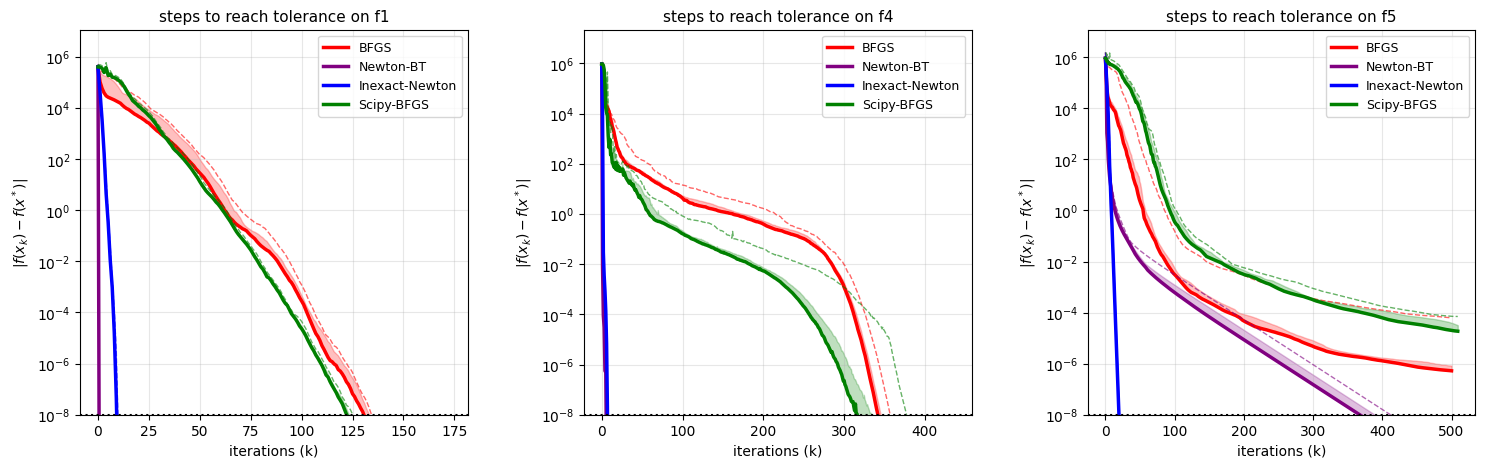
\includegraphics[width=\textwidth]{iterations_plot.png}
    \caption{Convergence in terms of iterations for $f_1$, $f_4$, and $f_5$. $d=200$, $\epsilon=1e-8$,$\rho=0.5$}
    \label{fig:iterations}
\end{figure}

\subsection{Performance Evaluation}

From Figure~\ref{fig:iterations} we observe that the inexact Newton method reaches the prescribed tolerance in the fewest iterations, followed by Newton with backtracking, while BFGS requires more iterations. This behaviour is consistent with the theoretical results in the notes. If the exact Hessian is used and the iterates remain in a neighbourhood of the solution, Newton’s method converges Q-quadratically locally. In contrast, BFGS achieves Q-superlinear convergence under suitable assumptions (Definition 2). Since quadratic convergence dominates superlinear convergence asymptotically, the Newton-type 
methods are expected to exhibit a steeper decrease close to the minimiser. This faster asymptotic rate is clearly visible in the iteration plots, where the Newton curves drop more sharply near the solution.
However, iteration counts alone do not determine practical efficiency. The computational cost per iteration must also be taken into account.

\subsection{Influence of Dimension and Computational Cost}

Figure~\ref{fig:time} shows the convergence behaviour for $f_5$ with respect to wall-clock time for $d=20$ and $d=500$. Exact Newton requires solving
\[
\nabla^2 f(x_k) p_k = -\nabla f(x_k)
\]
which for Newton's method has computational complexity $\mathcal{O}(n^3)$ due to the linear system solve. In contrast, BFGS, like inexact Newton, avoids explicit second derivatives and updates a dense matrix approximation using rank-two updates, leading to $\mathcal{O}(n^2)$ cost per iteration.

\begin{figure}[H]
    \centering
    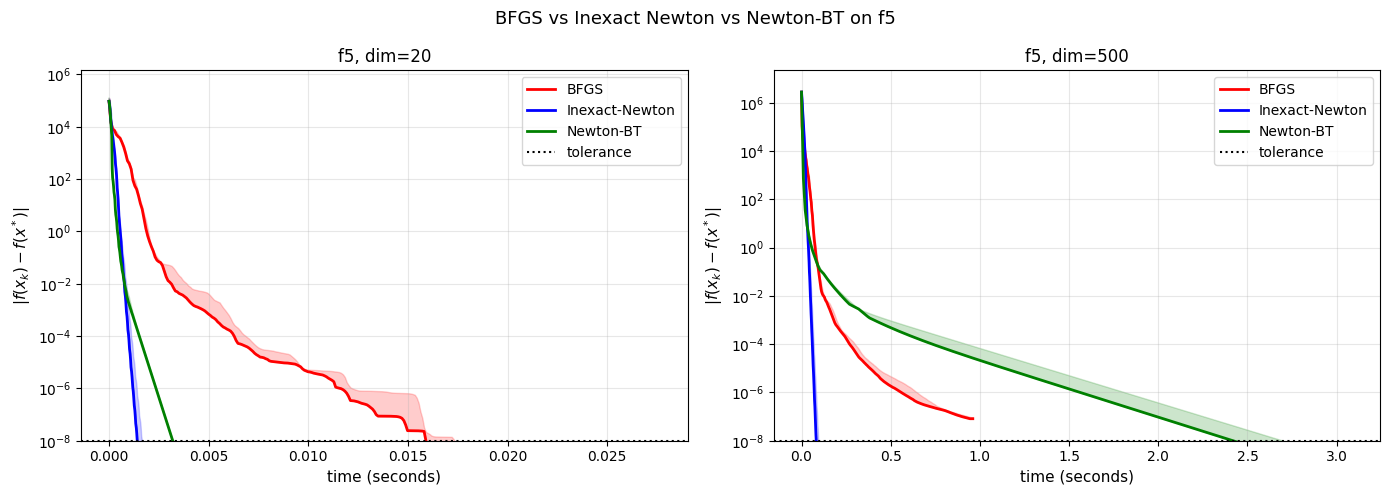
\includegraphics[width=0.75\textwidth]{time_plot.png}
    \caption{Convergence in wall-clock time for $f_5$ with $d=20$ and $d=500$, $\epsilon=1e-8$, $\rho=0.5$}
    \label{fig:time}
\end{figure}

\subsection{Competitiveness of BFGS}

The experiments demonstrate that BFGS is robust and does not require explicit Hessian information, which makes it attractive when second derivatives are unavailable, expensive, or when the Hessian is not positive definite. In contrast, Newton's method requires a positive definite Hessian to guarantee a descent direction. This observation is consistent with the theory in the notes. Newton’s Q-quadratic local convergence explains its rapid decrease near the minimiser, while the Q-superlinear convergence of BFGS accounts for its slightly slower asymptotic behaviour. The experiments confirm that practical performance depends not only on convergence rate but also crucially on per-iteration computational complexity and structure of the Hessian.

\section{Conclusion}

The analysis shows that BFGS achieves Q-superlinear convergence while Newton’s method retains Q-quadratic local convergence. The numerical results confirm this behaviour and highlight the trade-off between convergence rate and per-iteration cost. In practice, BFGS is a robust and competitive alternative when second derivatives are unavailable or expensive.

\end{document}
